\documentclass[a4paper,12pt,twoside]{article}
%\usepackage{mathpazo}
\usepackage{amsmath} % จะใช้ package ของ math อื่นใด ให้เรียกก่อน fontspec
\usepackage{amssymb} % จะใช้ package ของ math อื่นใด ให้เรียกก่อน fontspec
\usepackage{amsfonts} % จะใช้ package ของ math อื่นใด ให้เรียกก่อน fontspec
\usepackage{mathspec} % เรียกใช้แค่นี้มีค่า = \usepackage[no-math]{fontspec}\usepackage{mathspec}
\usepackage{xunicode,xltxtra}
\XeTeXlinebreaklocale "th"
\XeTeXlinebreakskip = 0pt plus 1pt %
\defaultfontfeatures{Scale=1.23}
\renewcommand{\baselinestretch}{1.2}
\setmainfont{TH Sarabun New}
\newfontfamily\kodchasal{TH Kodchasal} % ตั้งชื่อฟอนต์ใหม่เพื่อให้ง่ายต่อการใช้งาน เผื่อว่าในเอกสารต้องการให้มีหลายฟอนต์ เวลาใช้ก็ {\examplefont ข้อความต่าง ๆ}
\newfontfamily\niramit{TH Niramit AS}
\usepackage{xcolor}
\definecolor{MyColor}{rgb}{0.3,0.4,0.5} % กำหนดสี และชื่อที่จะใช้เรียกสีโดย xcolor
\everymath{\displaystyle} % บังคับให้ทุกสมการเป็น displaystyle
\usepackage{tabls}
\usepackage{graphicx}
\usepackage{tabularx}
\usepackage{booktabs}
\usepackage{longtable}
\usepackage{wrapfig} %ตัวหนังสือล้อมรอบรูปหรือตารางได้ (wrapfigure,wraptable) *** ไม่สามารถอยู่ในพวก enumerate ได้
\usepackage[Glenn]{fncychap}
\usepackage{sectsty,ulem}
\allsectionsfont{\ulemheading{\uline}}
\makeatletter
\def\@seccntformat#1{\csname the#1\endcsname)\quad}
\makeatother
\usepackage{cellspace}
\usepackage[usenames,dvipsnames]{pstricks} 
\usepackage{epsfig} 
\usepackage{pst-grad} % For gradients
\usepackage{pst-plot} % For axes 
\usepackage{makecell}
\usepackage{fancyhdr}
\usepackage{lastpage}
\usepackage{fancybox}
\usepackage{multirow}
\usepackage{calc}
% ระยะช่องว่างหน้า+หลังเลขหรืออักษรในสมการ หน่วยเป็น mmu , 1 mmu = 1mu/1000 , 18mu = 1 em ,default = 500 mmu = 1/36 em 
% ตัวไหนจะให้มีระยะพิเศษก็ใส่ " นำหน้า เช่น $ x^{"2} หรือใส่ทีละคำให้ใส่เป็น $ x^{\"3yz"} $
% \setminwhitespace[XXXX] 
\setminwhitespace[3000] 

% เลือก Math Font ต่าง ๆ นา ๆ
%\setmathsfont(Digits,Latin){Asana Math}
%\setmathsfont(Digits,Latin){jsMath-cmr10}
%\setmathsfont(Digits,Latin){Kerkis}
%\setmathsfont(Digits,Latin){Neo Euler}
%\setmathsfont(Digits,Latin){Fontin}
%\setmathsfont(Digits,Latin){Plakken}
%\setmathsfont(Digits,Latin){DejaVu Serif}
%\setmathsfont(Digits,Latin){STIXGeneral}
%\setmathsfont(Digits,Latin){CMU Bright}
%\setmathsfont(Digits,Latin){Iwona Light}
%\setmathsfont(Digits,Latin,Greek)[Numbers={Lining,Proportional}]{Iwona Light}
%\setmathsfont(Digits,Latin,Greek){TH Sarabun New}
%\setmathsfont(Digits,Latin,Greek){Mathmos Original}
% ใช้ฟอนต์ OTF ในเอกสารแต่ MATH ใช้ฟอนต์ Math
%\usepackage[no-math]{fontspec}

% ใช้ฟอนต์ OTF ในเอกสารและ MATH ใช้ฟอนต์ OTF
%\usepackage[no-math]{fontspec}
%\usepackage{mathspec}
%\setmainfont{TH Sarabun New}
%\setallmainfonts(Digits,Latin,Greek){TH Sarabun New}
\setallmainfonts(Digits,Latin,Greek){TH Sarabun New}

% \setmathrm จะเปลี่ยนฟอนต์เฉพาะที่อยู่ในคำสั่ง \mathrm{.....} เท่านั้น
%\setmathrm{TH Sarabun New}
%\setmathsfont(Digits,Latin,Greek){TH Sarabun New}
%\setmathfont(Digits,Latin,Greek){TH Sarabun New}

%\usepackage[top=1in,bottom=1in,left=1.2in,right=2in,showframe]{geometry}
%\usepackage[top=1in,bottom=1in,left=1.2in,right=2in]{geometry}
\usepackage{lipsum}
\usepackage{marginnote}
\usepackage[top=1in,bottom=1in,outer=2in,inner=1.2in,heightrounded,marginparwidth=1.5in,marginparsep=0.5in]{geometry}
\usepackage{paralist}
%\usepackage{auto-pst-pdf,pst-barcode}
\usepackage{pst-barcode}
\usepackage{blindtext}
\pagestyle{fancy}
\special{papersize=\the\paperwidth,\the\paperheight}
\usepackage{enumitem} % ใช้ rusume ได้ ไม่ต้อง setcounter

%\setlength\parindent{0pt}

\fancyhead[L]{ติวสบายฟิสิกส์}
\fancyhead[R]{www.pec9.com}
%\fancyfoot[L]{\begin{pspicture}(1in,1in)
%        \psbarcode{http://books.educasy.com/p/p000001}{eclevel=L}{qrcode}
%    \end{pspicture}}
\begin{document}
\begin{enumerate}%[leftmargin=12pt]
	\item \ovalbox{\textbf{p000001}} วัตถุหนึ่งเคลื่อนที่เป็นวงกลมรัศมี   14  เมตรครบหนึ่งรอบ   การกระจัดมีค่าเท่าใด \\ 
		1.  0  เมตร	\hfill			2.  14  เมตร		\hfill\phantom{xx} \\
		3.  44  เมตร		\hfill		4.  88   เมตร \hfill\phantom{xx}
\vspace{0.8in}
\end{enumerate}

\marginnote{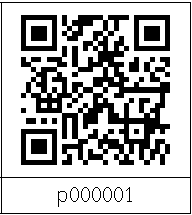
\includegraphics{p000001.pdf}}[-2.2in]
\marginnote{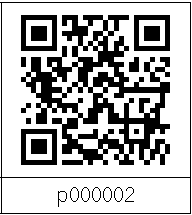
\includegraphics{p000002.pdf}}[-0.2in]
\marginnote{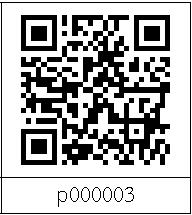
\includegraphics{p000003.pdf}}[1.8in]
\marginnote{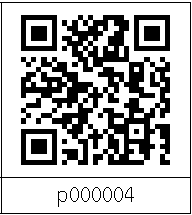
\includegraphics{p000004.pdf}}[3.8in]

\begin{center}\fbox{\begin{minipage}{0.8\textwidth}
\textbf{อัตราเร็วเฉลี่ย} หาค่าได้จากอัตราส่วนระหว่างระยะทางที่เคลื่อนที่ได้กับเวลาที่ในการเคลื่อนที่ช่วงนั้น  มีหน่วยเป็นเมตรต่อวินาที ( m/s ) นั่นคือ       
$$
\text{อัตราเร็วเฉลี่ย} = \frac{\text{ระยะทางที่เคลื่อนที่ได้}}{\text{เวลาที่ใช้}}
$$
\textbf{ความเร็วเฉลี่ย} หาค่าได้จากอัตราส่วนระหว่างการกระจัดของเคลื่อนที่กับเวลาที่ในการเคลื่อนที่ช่วงนั้น  มีหน่วยเป็นเมตรต่อวินาที ( m/s ) นั่นคือ
$$
\text{ความเร็วเฉลี่ย} = \frac{\text{การกระจัด}}{\text{เวลาที่ใช้}}
$$
\hfill \ovalbox{\textbf{p000002}}
\end{minipage}
}\end{center}

\begin{enumerate}[resume]
%\setcounter{enumi}{1}
	\item \ovalbox{\textbf{p000003}} \textbf{(แนว O-Net})  เด็กคนหนึ่งวิ่งเป็นเส้นตรงไปทางขวา  10  เมตรในเวลา  3  วินาที   จากนั้นก็หันกลับแล้ววิ่งเป็นเส้นตรงไปทางซ้ายอีก   5  เมตรในเวลา   2  วินาที   อัตราเร็วเฉลี่ยของเด็กคนนี้เป็นไปตามข้อใด \\
		1.  1.0  เมตรต่อวินาที	\hfill							2.  3.0  เมตรต่อวินาที \hfill\phantom{xx}\\
		3.  5.0  เมตรต่อวินาที	\hfill							4.  7.5  เมตรต่อวินาที \hfill\phantom{xx}
\vspace{0.8in}
\end{enumerate}
\begin{enumerate}[resume]
%\setcounter{enumi}{2}
	\item \ovalbox{\textbf{p000004}} \textbf{(แนว O-Net)}  จากข้อที่ผ่านมา  ขนาดของความเร็วเฉลี่ยของเด็กคนนี้เป็นไปตามข้อใด  \\
		1.  1.0  เมตรต่อวินาที	\hfill							2.  3.0  เมตรต่อวินาที \hfill\phantom{xx}\\
		3.  5.0  เมตรต่อวินาที	\hfill							4.  7.5  เมตรต่อวินาที \hfill\phantom{xx}
\vspace{0.8in}
\end{enumerate}

\newpage

\begin{enumerate}[resume]
%\setcounter{enumi}{3}
	\item \textbf{(แนว O–net)}  ตอนเริ่มต้นวัตถุอยู่ห่างจากจุดอ้างอิงไปทางขวา  2.0  เมตร   เมื่อเวลาผ่านไป  10  	วินาที   พบว่าวัตถุอยู่ห่างจากจุดอ้างอิงไปทางซ้าย   3.0  เมตร  จงหาความเร็วเฉลี่ยของวัตถุนี้ \\
 		 1.  0.5  เมตรต่อวินาที 	 ทางขวา	\hfill	 			2.  0.5  เมตรต่อวินาที  ทางซ้าย \hfill\phantom{xx}\\
 		 3.  1.0  เมตรต่อวินาที 	 ทางขวา	\hfill	  			4.  1.0  เมตรต่อวินาที  ทางซ้าย \hfill\phantom{xx}
\vspace{0.8in}
\end{enumerate}

\begin{enumerate}[resume]
%\setcounter{enumi}{4}
	\item \ovalbox{\textbf{p000005}} \textbf{(แนว มช)}  รถโดยสารเริ่มออกเดินทางจากกรุงเทพฯเวลา   22.00  น.   มาถึงเชียงใหม่เวลา 8.00 น. กำหนดให้ระยะทางจากกรุงเทพฯถึงเชียงใหม่เป็น   720  กิโลเมตร   จงหาว่ารถโดยสารคันนี้วิ่งด้วยอัตราเร็วเฉลี่ยเท่าใด \\
		1.  10  กิโลเมตรต่อชั่วโมง		\hfill					2.  100  กิโลเมตรต่อชั่วโมง \hfill\phantom{xx}\\
		3.  72  กิโลเมตรต่อชั่วโมง		\hfill					4.  720  กิโลเมตรต่อชั่วโมง \hfill\phantom{xx}
\vspace{0.8in}
\end{enumerate}

\begin{center}\fbox{\begin{minipage}{0.8\textwidth}
กรณีที่วัตถุเคลื่อนที่ไปด้วยความเร็วคงที่   จะได้ว่า 
	\begin{align*}
		\text{ระยะทางที่เคลื่อนที่ได้}  &=  \text{อัตราเร็ว}\times \text{เวลาที่ใช้เคลื่อนที่} \\
		\text{\textbf{หรือ}}\qquad \qquad			  s  &=  v \cdot  t
	\end{align*}
	\begin{tabbing}
						\textbf{เมื่อ} \quad  \=\textbf{s}  คือระยะทางที่เคลื่อนที่ได้ \quad \=หน่วยเป็นเมตร ( m ) \\
							  				\>\textbf{v}  คืออัตราเร็วซึ่งคงที่  \> หน่วยเป็นเมตรต่อวินาที ( m/s ) \\
							   				\>\textbf{t}  คือเวลาที่ใช้เคลื่อนที่  \> หน่วยเป็นวินาที ( s )
	\end{tabbing}
\hfill \ovalbox{\textbf{p000006}}
\end{minipage}
}
\end{center}

\begin{enumerate}[resume]
%\setcounter{enumi}{5}
\setlength{\leftmargin}{0pt}
\item รถยนต์คันหนึ่งวิ่งด้วยอัตราเร็วคงตัว   15  เมตรต่อวินาทีเป็นเวลานาน  60  วินาที  	ระยะทางที่รถยนต์คันนี้เคลื่อนที่ได้จะมีขนาดเท่ากับข้อใดต่อไปนี้ \\
		1.  45  m		\hfill			2.  90  m			\hfill\phantom{xx}\\		
		3.  450  m	\hfill				4.   900  m \hfill\phantom{xx}
\vspace{0.8in}
\end{enumerate}

\marginnote{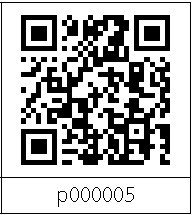
\includegraphics{p000005.pdf}}[-8.7in]
\marginnote{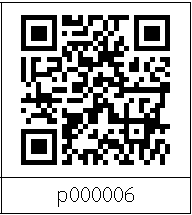
\includegraphics{p000006.pdf}}[-6.7in]

\end{document}

